\documentclass[a4j,10pt]{jarticle}
\usepackage[dvipdfmx]{graphicx}
\begin{document}
  \section{実験の目的}
  ガイガー・ミューラー計数管(以下,GM計数管と記す)を利用して放射線元素の崩壊の法則と物質による放射線の吸収について調べる.
  \section{実験の原理}
  \subsection{放射性元素の崩壊}
  原子核は陽子と中性子からなっている.原子核には不安定なものがあり,それらが崩壊して$\alpha$線(Heの原子核)や$\beta$線(電子),$\gamma$線(電磁波)を放出し安定した原子核になる.
  このことを放射性元素の崩壊と呼ぶ.

  今回の実験で用いる放射性源である${}^{137}_{55}$Cs(セシウム137)は
  \begin{eqnarray}
    \label{cs}
    {}_{55}^{137}\mathrm{Cs} \rightarrow {}_{56}^{137}\mathrm{Cs} + \mathrm{e}^{-} + \bar{\nu}_e
  \end{eqnarray}
  (\ref{cs})のように電子$\mathrm{e}^{-}$と中性微子$\bar{\nu}_e$を放出して、${}_{56}^{137}$H(バリウム137)に崩壊する.
  このことを$\beta-$崩壊という.

  \subsection{$\beta$線の吸収}
  $\beta$線が物質を通過するとき,エネルギーを失い減衰していく.
  $\beta$線の電子$N$個が厚さ$\mathrm{d}x$の物質の層を通過する間に吸収されて減衰する割合$\mathrm{d}N/\mathrm{d}x$は電子数$N$に比例し,比例定数を$\mu$(線吸収係数)を用いると
  \begin{eqnarray}
    \label{beta}
    \frac{\mathrm{d}\mathcal{N}}{\mathrm{d}x} = -\mu \mathcal{N}
  \end{eqnarray}
  (\ref{beta})と表すことができる.
  物質に入射前に$\mathcal{N}_0$個の電子があったとすれば、厚さ$x$の物質層を通過して出てくる電子数は
  \begin{eqnarray}
    \label{nx}
    \mathcal{N}(x)=\mathcal{N}_0 \mathrm{e}^{-\mu x}
  \end{eqnarray}
  となる.
  物質層の厚さ$x$の代わりに単位面積当たりの質量$\rho_s$($=\rho x$:$\rho$は密度),$\mu$の代わりに質量吸収係数$\mu_m(=\mu/\rho)$を用いると,(\ref{nx})は
  \begin{eqnarray}
    \mathcal{N}(x)=\mathcal{N}_0 \mathrm{e}^{-\mu_m \rho_s}
  \end{eqnarray}
  と表すことができる.

  \section{実験の方法}
  \subsection{自然係数の測定}
  放射線源がない状態でGM計数管のスタンドに何も入れないで,GM計数管の電源を入れた.
  計測時間を60 sにセットして60 sの間の係数を合計20回測定した.

  \subsection{$\beta$線の吸収係数の観測}
  GM計数管のスタンドの60 mmのところに放射線源をいれ,その上の50 mmのところに中央に直径28.8 mmの穴の開いた板を入れた。計測時間を60 sにセットして以下の3つの測定をした.
  \begin{enumerate}
    \item そのままの状態で,1分間の計数値$N$を求めた.
    \item 厚さ1mmのAl板で50mmの段の板の穴を塞ぎ,1分間の計数値$N'$を求めた.
    \item Al板を取り出し,Cu薄板を0枚から1枚ずつ(最大5枚)入れていき,各枚数の時の計数値$N_1$を測定した.
    \item Tiを0枚から1枚ずつ(最大6枚)入れていき,各枚数の時の計数値$N_2$を測定した.
  \end{enumerate}
  これらをそれぞれ5回繰り返し計測した.
  \section{結果}
  \subsection{自然計数の測定結果}
  自然計数の測定は20回行った.その測定結果は(\ref{nt})のようになった.自然計数の平均$\overline{N}_0$は、$\overline{N}_0=14.7$と求められた。

        \begin{table}[h]
          \label{nt}
          \begin{center}
            \caption{自然計数の測定結果}
              \begin{tabular}{cc}
                \hline
                計数値 & 出現回数 \\ \hline
                8 & 2 \\
                11 & 2 \\
                12 & 1 \\
                13 & 3 \\
                14 & 2 \\
                15 & 1 \\
                16 & 3 \\
                18 & 2 \\
                19 & 2 \\
                20 & 2 \\
                \hline
              \end{tabular}
            \end{center}
        \end{table}

  また横軸に計数値$N$,縦軸に計数値$N$の出現回数$n$をとった棒グラフを図1にまとめた.
  \begin{figure}[htbp]
    \begin{center}
    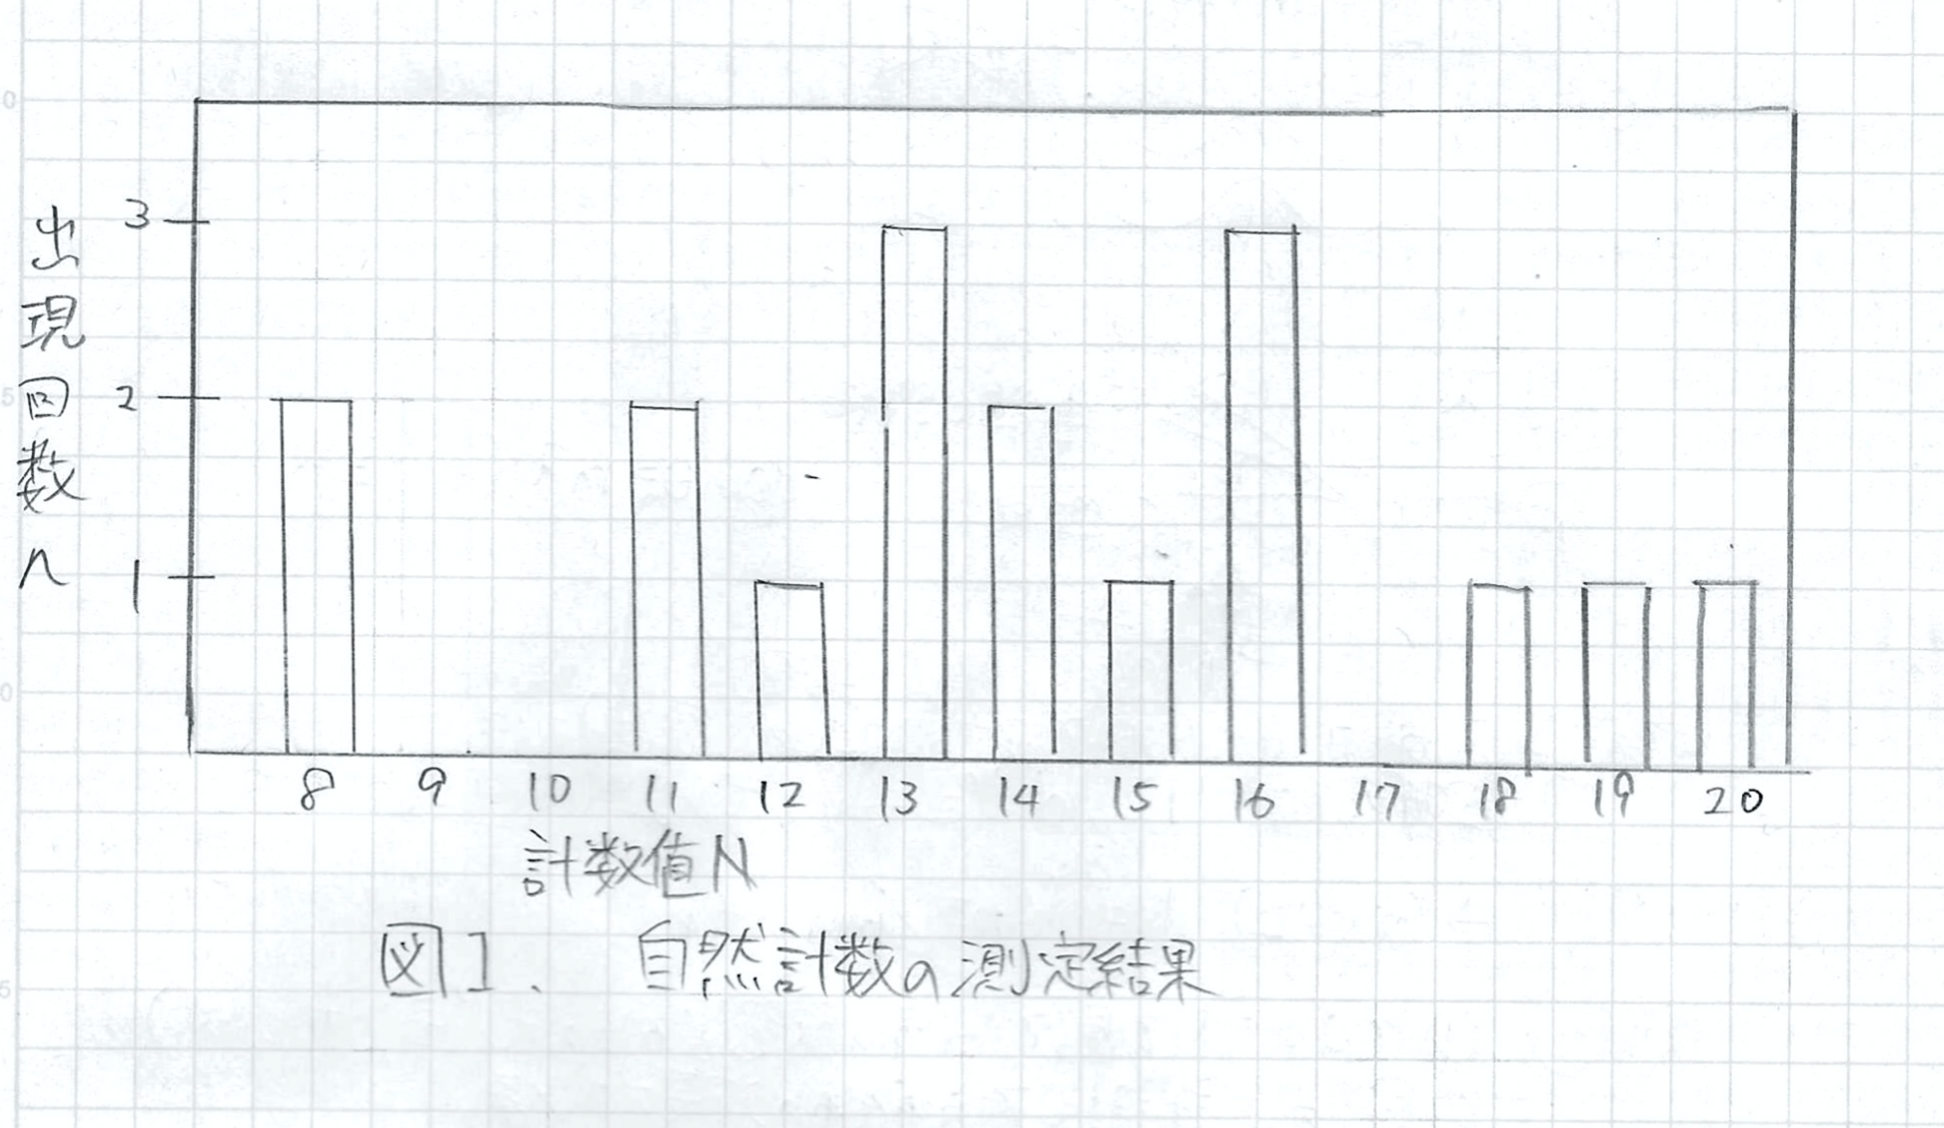
\includegraphics[width=100mm]{sizen.png}
    \caption{自然係数の測定結果}
    \end{center}
  \end{figure}
  \subsection{$\beta$線の吸収係数の測定結果}
  まずは.穴の開いた板のみの場合を測定した.
  \begin{table}[h]
    \begin{center}
      \caption{$N$の測定結果}
        \begin{tabular}{c|cccccccccc}
          \hline
          測定回数 & 1 & 2 & 3 & 4 & 5  \\ \hline
          $N$ & 492 & 516 & 518 & 499 & 505 \\
          \hline
        \end{tabular}
    \end{center}
  \end{table}
    この平均$\overline{N}$は$\overline{N}=506$と求められた.
  次に,厚さ1mmのAl板を入れたときについて,計数値$N'$の測定結果は次のようになった.

  \begin{table}[h]
    \begin{center}
      \caption{$N'$の測定結果}
        \begin{tabular}{c|cccccccccc}
        \hline
        測定回数 & 1 & 2 & 3 & 4 & 5  \\ \hline
        $N'$ & 115 & 138 & 143 & 125 & 114 \\
        \hline
        \end{tabular}
      \end{center}
    \end{table}
    
  この平均$\overline{N'}$は$\overline{N'}=127$となった.
  この2つの結果より,$\beta$線の計数値の平均値$\overline{N_\beta}$は
  \begin{eqnarray}
    \overline{N_\beta} = \overline{N} - \overline{N'}
  \end{eqnarray}
  より$\overline{N_\beta}=379$となった.
    \subsubsection{Cu板による吸収の測定結果}
      5枚のCu板の厚さとその平均値は表4のようになった.
    \begin{table}[h]
      \label{Cuatusa}
      \begin{center}
      \caption{Cu板の厚さの測定結果}
        \begin{tabular}{ccccccc}
        \hline
        n番目に使ったCu板&\multicolumn{5}{c}{測定回数$/\mathrm{mm}$} & 平均$/\mathrm{mm}$ \\
          & 1 & 2 & 3 & 4 & 5 & \\ \hline
        1 & 0.007 & 0.001 & 0.008 & 0.006 & 0.008 & 0.006 \\
        2 & 0.004 & 0.003 & 0.007 & 0.006 & 0.007 & 0.0054\\
        3 & 0.005 & 0.003 & 0.008 & 0.004 & 0.008 & 0.0056\\
        4 & 0.008 & 0.002 & 0.003 & 0.001 & 0.002 & 0.0032\\
        5 & 0.001 & 0.002 & 0.003 & 0.005 & 0.003 & 0.0028\\
        \hline
        \end{tabular}
      \end{center}
    \end{table}
    $\beta$線源の位置60 mm,金属板の位置50 mm,計数時間60 sで行った.Cu板の枚数を変えて測定した計数値$N$の結果とその平均値$\overline{N}$,$\beta$線の計数値$\overline{N}_{\beta}$とその対数,標準偏差$\sigma_{\beta}$、$\log_{\mathrm{e}}(\overline{N}_{\beta}-\sigma_{\beta})$と$\log_{\mathrm{e}}(\overline{N}_{\beta}+\sigma_{\beta})$の計算結果を次の表にまとめた.なお,標準偏差$\sigma_{\beta}$は,各測定の繰り返しの回数$n$として次のように求めた.
    \begin{eqnarray}
      \sigma_{\beta} = \sqrt{\frac{\overline{N}+\overline{N'}}{n}}
    \end{eqnarray}
    これらをまとめたのが表5である.
    \begin{table}[h]
      \label{Cukeisoku}
      \begin{center}
      \caption{Cu板における$\beta$線の吸収の測定結果}
      \scalebox{0.6}[0.9]{
        \begin{tabular}{ccccccccc}
        \hline
        枚数 & 厚さ$/\mathrm{mm}$ & $N$ & $\overline{N}$ & $\overline{N}_{\beta}$ & $\log_{\mathrm{e}}\overline{N}_{\beta}$ & $\sigma_{\beta}$ & $\log_{\mathrm{e}}(\overline{N}_{\beta}-\sigma_{\beta})$ & $\log_{\mathrm{e}}(\overline{N}_{\beta}+\sigma_{\beta})$ \\ \hline
        1 & 0.007 & 439,413,430,434,425 & 428.2 & 301.2& ¥5.7089 & 10.5476 & 39.2627 & 40.6638 \\
        2 & 0.011 & 388,363,398,372,373 & 379.6 & 252.6 & ¥5.5427 & 10.0658 & 35.8658 & 37.3247 \\
        3 & 0.016 & 282,310,311,262,303 & 293.6 & 166.6 & ¥5.1166 & 9.1715 & 28.8407 & 30.5329 \\
        4 & 0.024 & 255,291,240,239,269 & 258.8 & 131.8 & ¥4.8821 & 8.7841 & 25,5433 & 27.3062 \\
        5 & 0.025 & 217,210,250,238,240 & 231 & 104 & ¥4.6452 & 8.4617 & 22.5104 & 24.4228 \\
        \hline
        \end{tabular}
      }
      \end{center}
    \end{table}
    \subsubsection{Ti板による吸収の測定結果}
    6枚のTi板の厚さとその平均値は表6のようになった.
  \begin{table}[h]
    \label{Tiatusa}
    \begin{center}
    \caption{Ti板の厚さの測定結果}
      \begin{tabular}{ccccccc}
      \hline
      n番目に使ったTi板&\multicolumn{5}{c}{測定回数$/\mathrm{mm}$} & 平均$/\mathrm{mm}$ \\
        & 1 & 2 & 3 & 4 & 5 & \\ \hline
      1 & 0.022 & 0.018 & 0.012 & 0.011 & 0.021 & 0.0017\\
      2 & 0.019 & 0.013 & 0.021 & 0.018 & 0.020 & 0.0018\\
      3 & 0.015 & 0.016 & 0.011 & 0.019 & 0.013 & 0.0015\\
      4 & 0.017 & 0.020 & 0.019 & 0.012 & 0.014 & 0.0016\\
      5 & 0.011 & 0.009 & 0.009 & 0.018 & 0.016 & 0.0013\\
      6 & 0.011 & 0.010 & 0.012 & 0.010 & 0.009 & 0.0010\\
      \hline
      \end{tabular}
    \end{center}
  \end{table}
  $\beta$線源の位置60mm,金属板の位置50mm,計数時間60sで行った.Ti板の枚数を変えて測定した計数値$N$の結果とその平均値$\overline{N}$,$\beta$線の計数値$\overline{N}_{\beta}$とその対数,標準偏差$\sigma_{\beta}$、$\log_{\mathrm{e}}(\overline{N}_{\beta}-\sigma_{\beta})$と$\log_{\mathrm{e}}(\overline{N}_{\beta}+\sigma_{\beta})$の計算結果を次の表にまとめた.なお,標準偏差$\sigma_{\beta}$は,各測定の繰り返しの回数$n$として次のように求めた.
  \begin{eqnarray}
    \sigma_{\beta} = \sqrt{\frac{\overline{N}+\overline{N'}}{n}}
  \end{eqnarray}
  これらをまとめたのが表7である.
  \begin{table}[h]
    \label{Tilkeisoku}
    \begin{center}
    \caption{Ti板における$\beta$線の吸収の測定結果}
    \scalebox{0.6}[0.9]{
      \begin{tabular}{ccccccccc}
      \hline
      枚数 & 厚さ$/\mathrm{mm}$ & $N$ & $\overline{N}$ & $\overline{N}_{\beta}$ & $\log_{\mathrm{e}}\overline{N}_{\beta}$ & $\sigma_{\beta}$ & $\log_{\mathrm{e}}(\overline{N}_{\beta}-\sigma_{\beta})$ & $\log_{\mathrm{e}}(\overline{N}_{\beta}+\sigma_{\beta})$ \\ \hline
      1 & 0.022 & 444,416,466,443,464 & 446.6 & 319.6 & ¥5.7681 & 27.6803 & 5.6776 & 5.8512 \\
      2 & 0.041 & 371,406,365,380,350 & 374.4 & 247.4 & ¥5.512 & 17.6324 & 5.4381 & 5.5809 \\
      3 & 0.056 & 316,279,343,309,336 & 316.6 & 189.6 & ¥5.2458 & 12.9897 & 5.1776 & 5.3121 \\
      4 & 0.073 & 260,276,291,273,240 & 268 & 141 & ¥4.9496 & 10.1119 & 4.8752 & 5.0189 \\
      5 & 0.084 & 238,234,259,252,260 & 248 & 121 & ¥4.7967 & 8.5907 & 4.7230 & 4.8653 \\
      6 & 0.095 & 217,210,200,211,213 & 210.2 & 83.2 & ¥4.4197 & 6.9929 & 4.3342 & 4.5949 \\
      \hline
    \end{tabular}
    }
    \end{center}
  \end{table}
  この結果より,片対数グラフを使用して図2に横軸が金属板の厚さ,縦軸に$\log_{10}\overline{N}_{\beta}$をとるグラフを作成した.
  図2から傾きを計算するとCu板${-1.12×10^3\,cm^-1}$,Ti板が${-3.095×10^4\,cm^-1}$となった.
  この値は線吸収係数$\mu$に等しい.
  Cuの密度は$\rho=8.96\,{\rm g}/{\rm cm}^3$,Tiの密度は$\rho=4.54\,{\rm g}/{\rm cm}^3$ \cite{f}より,
  Cuの質量吸収線係数$\mu_{\rm m}$は
  \begin{equation}
    \mu_{\rm m} = \frac{\mu}{\rho} = \frac{112}{8.96} = 12.5... \cong 12.5\,{\rm cm}^2/{\rm g}
  \end{equation} 
  Tiの質量吸収線係数$\mu_{\rm m}$は
  \begin{equation}
    \mu_{\rm m} = \frac{\mu}{\rho} = \frac{3095}{4.54} = 681.718... \cong 681.72 \,{\rm cm}^2/{\rm g}
  \end{equation}
  と求められた.
  

  \section{考察}
  自然係数の測定結果の図1の棒グラフを見て,現在の計測回数ではポアソン分布らしき形はしている.計測回数をもっと増やしていくとポアソン分布に収束していくと考えられる.
  
  $\beta$線の吸収の測定結果によるとCu板の方が厚さあたりの吸収量が多いことがわかった.
  \begin{thebibliography}{9}
    \bibitem{kiso} 電気通信大学,『基礎物理学実験』2021年 p66$\sim$76
    \bibitem{f} 国立天文台『理科年表』2022年
    \end{thebibliography}
    \end{document}
  \end{document}